\subsection{Conmutación de Circuitos}

La conmutación de circuitos es la tecnología tradicional de la red telefónica pública. En este esquema, se establece un camino de comunicación dedicado entre dos estaciones a través de los nodos de la red. Este vínculo físico o canal lógico se mantiene de forma exclusiva para esa conexión específica, lo que garantiza:

\begin{itemize}
	\item \textbf{Reserva de recursos}: El ancho de banda y la capacidad de conmutación se reservan íntegramente para el par de usuarios.
	\item \textbf{Transparencia}: Una vez establecido el circuito, la red opera de forma invisible, permitiendo una transmisión continua sin retardos de procesamiento adicionales.
	\item \textbf{Capacidad fija}: Los datos fluyen a una velocidad constante, limitada únicamente por el tiempo de propagación de la señal.
\end{itemize}

El encaminamiento en estas redes se gestiona en tres fases críticas:

\begin{enumerate}
	\item \textbf{Establecimiento del circuito}: Se determina y activa el camino de extremo a extremo, realizando reservas de canales en cada nodo intermedio.
	\item \textbf{Transferencia de datos}: La información fluye libremente por el camino dedicado.
	\item \textbf{Desconexión}: Se liberan los recursos reservados para que puedan ser utilizados por otros usuarios.
\end{enumerate}

\subsection{Encaminamiento Jerárquico (Estático)}

En una red de conmutación de circuitos de gran escala, las conexiones suelen requerir una ruta que atraviese múltiples conmutadores. Para gestionar esto, la arquitectura de red debe equilibrar dos requisitos fundamentales:

\begin{itemize}
	\item \textbf{Eficiencia}: Consiste en minimizar la cantidad de equipos (conmutadores y enlaces) necesarios para gestionar la carga esperada. Esta carga, denominada \textbf{tráfico}, se define como el promedio de uso durante los periodos de mayor actividad.
	\item \textbf{Flexibilidad}: Es la capacidad de la red para proporcionar un servicio aceptable incluso ante condiciones adversas, como fallos en nodos o picos inesperados de demanda.
\end{itemize}

\begin{figure}[H]
	\centering
	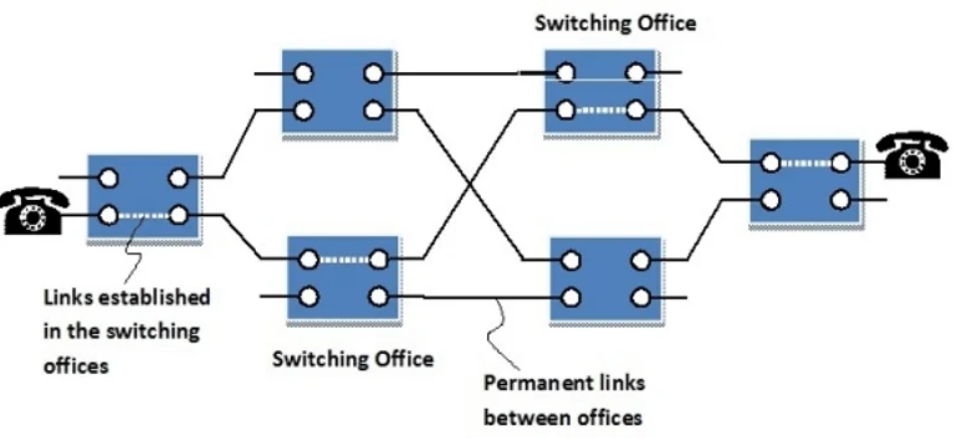
\includegraphics[width=0.8\textwidth]{img/Circuitos.png}
	\caption{Red de conmutación de circuito}
	\label{fig:grafico1}
\end{figure}

Tradicionalmente, la función de encaminamiento se ha basado en una estructura de \textbf{árbol o jerarquía}. Las rutas se establecen desde el emisor hacia un nodo común superior y luego descendiendo hacia el receptor. Aunque este esquema es simple de implementar, presenta limitaciones críticas: la eficiencia se ve comprometida al tener que dimensionar la red para picos de carga fijos, y la flexibilidad es escasa, ya que una estructura jerárquica rígida responde pobremente ante fallos en los niveles superiores del árbol.

Para mitigar estas carencias, a menudo se añaden enlaces de alta capacidad fuera de la jerarquía estricta para aportar redundancia, aunque sin alcanzar la adaptabilidad de los esquemas dinámicos.

\begin{figure}[H]
	\centering
	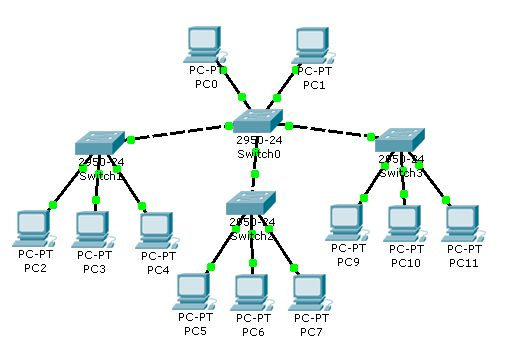
\includegraphics[width=0.5\textwidth]{img/arbol.jpg}
	\caption{Topología de árbol o jerárquica}
	\label{fig:grafico2}
\end{figure}

\subsection{Encaminamiento Alternativo y Dinámico}

A diferencia del modelo jerárquico, en un \textbf{esquema de encaminamiento dinámico} las decisiones se ven influenciadas por las condiciones de tráfico en tiempo real. En esta arquitectura, los nodos mantienen una relación de \textbf{igual a igual} (peer-to-peer), donde todos están capacitados para realizar las mismas funciones. Aunque esto aumenta la complejidad, proporciona una flexibilidad significativamente mayor al habilitar múltiples rutas alternativas.

La base de estos esquemas reside en el \textbf{encaminamiento alternativo}, donde el conmutador de origen selecciona la mejor ruta de un conjunto predefinido para cada llamada. Habitualmente, cada nodo dispone de una lista de rutas prefijadas en orden de preferencia: si la ruta directa está congestionada o no disponible, se intenta con la siguiente opción. Dependiendo de la variabilidad de estas listas, distinguimos dos tipos:

\begin{itemize}
	\item \textbf{Encaminamiento alternativo fijo}: Se utiliza una única secuencia de rutas predefinida, sin cambios a lo largo del día.
	\item \textbf{Encaminamiento alternativo dinámico}: Se emplean diferentes conjuntos de rutas según la franja horaria o el estado de la red. Esto permite aprovechar tanto los patrones de tráfico conocidos como las variaciones en el estado actual para optimizar el uso de los recursos globales.
\end{itemize}